\begin{frame}{Policy Simulation 1: Speed-up vs. Compensation}
    \begin{center}
        \textbf{Reducing delay can outperform compensation when delay costs are high.}
    \end{center}

    \vspace{1em}

    \begin{columns}[c]
        \begin{column}{0.65\textwidth}
            \begin{center}
                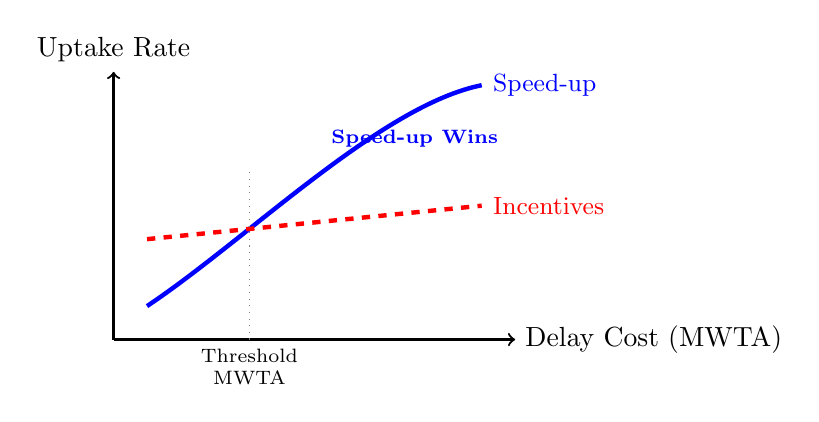
\begin{tikzpicture}[scale=0.85]
                    % Axes
                    \draw[thick,->] (0,0) -- (6,0) node[right] {Delay Cost (MWTA)};
                    \draw[thick,->] (0,0) -- (0,4) node[above] {Uptake Rate};
                    
                    % Speed-up Strategy (Rising)
                    \draw[blue, ultra thick] (0.5,0.5) .. controls (2,1.5) and (4,3.5) .. (5.5,3.8) 
                        node[right, font=\small] {Speed-up};
                    
                    % Compensation Strategy (Flat/Slow)
                    \draw[red, ultra thick, dashed] (0.5,1.5) -- (5.5,2.0) 
                        node[right, font=\small] {Incentives};
                    
                    % Break-even annotation
                    \draw[gray, thin, dotted] (2.03,0) -- (2.03,2.5);
                    \node[below, font=\scriptsize, text width=2cm, align=center] at (2.03,0) {Threshold MWTA};
                    
                    % High Efficiency Zone
                    \node[blue, font=\bfseries\scriptsize] at (4.5,3.0) {Speed-up Wins};
                \end{tikzpicture}
            \end{center}
        \end{column}
        
        \begin{column}{0.35\textwidth}
            \begin{itemize}
                \item \textbf{Speed-up} is most effective when delay costs are high
                \item \textbf{Incentives} preferred when speed-up is costly
            \end{itemize}
        \end{column}
    \end{columns}

    \vfill
    \begin{center}
        \textit{\textbf{Policy choice} depends on the relative cost of time vs. incentives.}
    \end{center}
\end{frame}
